\section{Blockchain}
\label{sec:blockchain}

La tecnologia \textit{Blockchain} è nota come \textit{registro distribuito}, essa consiste in una rete peer-to-peer di computer collocati globalmente che, grazie ad un meccanismo di consenso decentralizzato, permette di creare un registro condiviso strutturato a blocchi, sicuro ed immutabile. \cite{binance-blockchain}

Nel seguente capitolo verranno approfonditi i termini sopra citati, in modo da comprendere meglio il funzionamento della tecnologia \textit{Blockchain}.

I computer che partecipano alla \textit{Blockchain}, chiamati \textit{nodi}, collaborano per creare e mantenere un registro condiviso, il quale contiene tutte le transazioni effettuate all'interno della rete. Il termine \textit{Blockchain} prende il nome dalla sua struttura, ovvero un registro organizzato in blocchi concatenati tra loro, come mostrato in figura \ref{fig:blockchain-hash}. \cite{binance-blockchain}.

Ogni blocco contiene diverse informazioni, tra cui il numero del blocco, la data di creazione, le transazioni effettuate e l'hash del blocco precedente. \cite{binance-block} 

Con il termine \textit{transazione} si intende lo spostamento di un asset, che può essere una valuta nativa della \textit{Blockchain} oppure un token. \cite{ibm-blockchain} 

Il valore di \textit{hash} è un insieme di tutte le informazioni presenti in un blocco che vengono crittografate tramite funzioni matematiche. Questo valore è cruciale, dal momento che permette di rendere i blocchi una vera e propria catena. Così come rende estremamente difficile la modifica della \textit{Blockchain}, poiché il tentativo di alterazione di una transazione comporterebbe la modifica dell'hash del blocco e di conseguenza di tutti i blocchi successivi. \cite{bitsmap-block}
Per esempio, facendo riferimento alla figura \ref{fig:blockchain-hash} se si volesse modificare una transazione presente nel blocco uno, si dovrebbe modificare anche l'hash del blocco due e dunque anche del blocco tre.

Nel momento in cui un blocco viene creato e confermato, come approfondito nel paragrafo \hyperref[sec:consensoDistribuito]{\textit{Meccanismi di consenso ditribuito}}, le informazioni interne ad esso diventano immutabili, cioè non modificabili. \cite{binance-block}

In aggiunta, essendo la \textit{Blockchain} distribuita e replicata tra i diversi nodi la sua sicurezza è garantita. Un tentativo di alterazione di un blocco in una copia della \textit{Blockchain} dovrebbe essere replicato anche in tutti gli altri nodi della rete per essere considerato valido. \cite{bitsmap-block}

Infatti, la tecnologia \textit{Blockchain} è definita come \textit{tamper proof} e \textit{tamper evident}, ciò significa che la tecnologia è resiliente alle manipolazioni e che un tentativo di manomissione risulterebbe evidente. \cite{coinmarket-tamperProof}

Entrando più in dettaglio sul componente nodo, le tipologie esistenti sono di vario tipo. Tuttavia, lo scopo di ciascun nodo è quello di partecipare in modo attivo all'elaborazione e convalidazione di nuovi blocchi. I nodi definiti come \textit{full node}  possiedono una copia dell'intera \textit{Blockchain}, all'interno del loro spazio su disco.
Una seconda tipologia di nodo, chiamato \textit{light node}, ha lo scopo di velocizzare la rete, invece di scaricare e possedere l'intera \textit{Blockchain} salva lo stretto necessario per elaborare le transazioni. \cite{originstamp-nodi}

I nodi sono una componente fondamentale della \textit{Blockchain}, in quanto le consentono di essere sistemi \textit{borderless} (senza confini imposti dall'uomo, come i vari confini nazionali) e senza necessità di un intermediario nelle operazioni svolte. \cite{binance-blockchain}

\begin{figure}[ht]
\centering
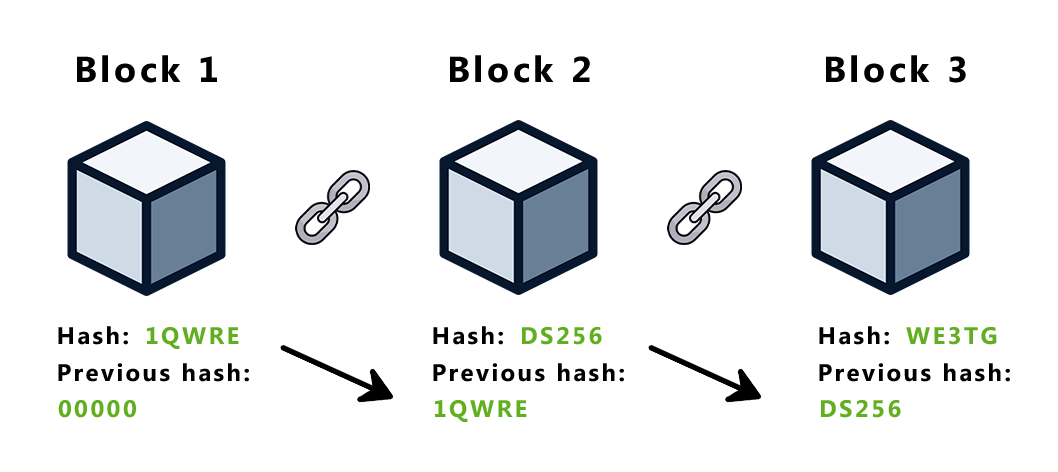
\includegraphics[scale=0.35]{images/blockchain-hash}
\caption{Connessione tra \emph{blocchi}}
\label{fig:blockchain-hash}
\end{figure}

Una fase chiave in una \textit{Blockchain} è concordare l'aggiunta di nuovi blocchi. Non essendoci un server centralizzato, saranno i nodi tramite un meccanismo di \textit{consenso distribuito}, come approfondito nel paragrafo \hyperref[sec:consensoDistribuito]{\textit{Meccanismi di consenso ditribuito}}, 
a validare un nuovo stato della blockchain basandosi sul sistema di \textit{Byzantine Fault Tolerance} (BFT).\cite{binance-bft}

In sintesi, la tecnologia \textit{Blockchain} rappresenta un registro distribuito sicuro e resiliente, la cui architettura decentralizzata e meccanismi di consenso la rendono un'innovazione significativa per numerose applicazioni.

\subsection{Wallet}
\label{sec:wallet}

Le maggiori \textit{Blockchain} come Bitcoin e Ethereum utilizzano un sistema crittografico con una coppia di chiave pubblica e privata. I \textit{wallet} sono dei sistemi che permettono agli utenti di interagire con le \textit{Blockchain} e quelli più utilizzati facilitano una serie di operazioni di comunicazione con le \textit{Blockchain}. \cite{ledger-privatekey}
        
La \textit{chiave privata} è segreta e viene utilizzata per generare la chiave pubblica. \cite{bitpanda-privatekey}

Come descritto nel capitolo \hyperref[sec:blockchain]{\textit{Blockchain}}, ogni blocco contiene diverse transazioni, che a loro volta contengono principalmente tre informazioni:
\begin{itemize}
    \item Un \textit{mittente}, il quale tramite la sua chiave privata cifra l'intera transazione. 
    \item L'indirizzo del \textit{destinatario}, che viene generato tramite la chiave pubblica.
    \item L'azione che vuole svolgere, per esempio il trasferimento di una criptovaluta.
\end{itemize}

Il meccanismo appena descritto può essere riassunto grazie alla Figura \ref{fig:privatePublicKeys}. \cite{ledger-privatekey}
Tramite la cifratura della transazione, la blockchain può verificare che il mittente sia l'unico con il diritto di richiedere l'operazione che vuole svolgere. \cite{bitpanda-privatekey}

\begin{figure}[ht]
\centering
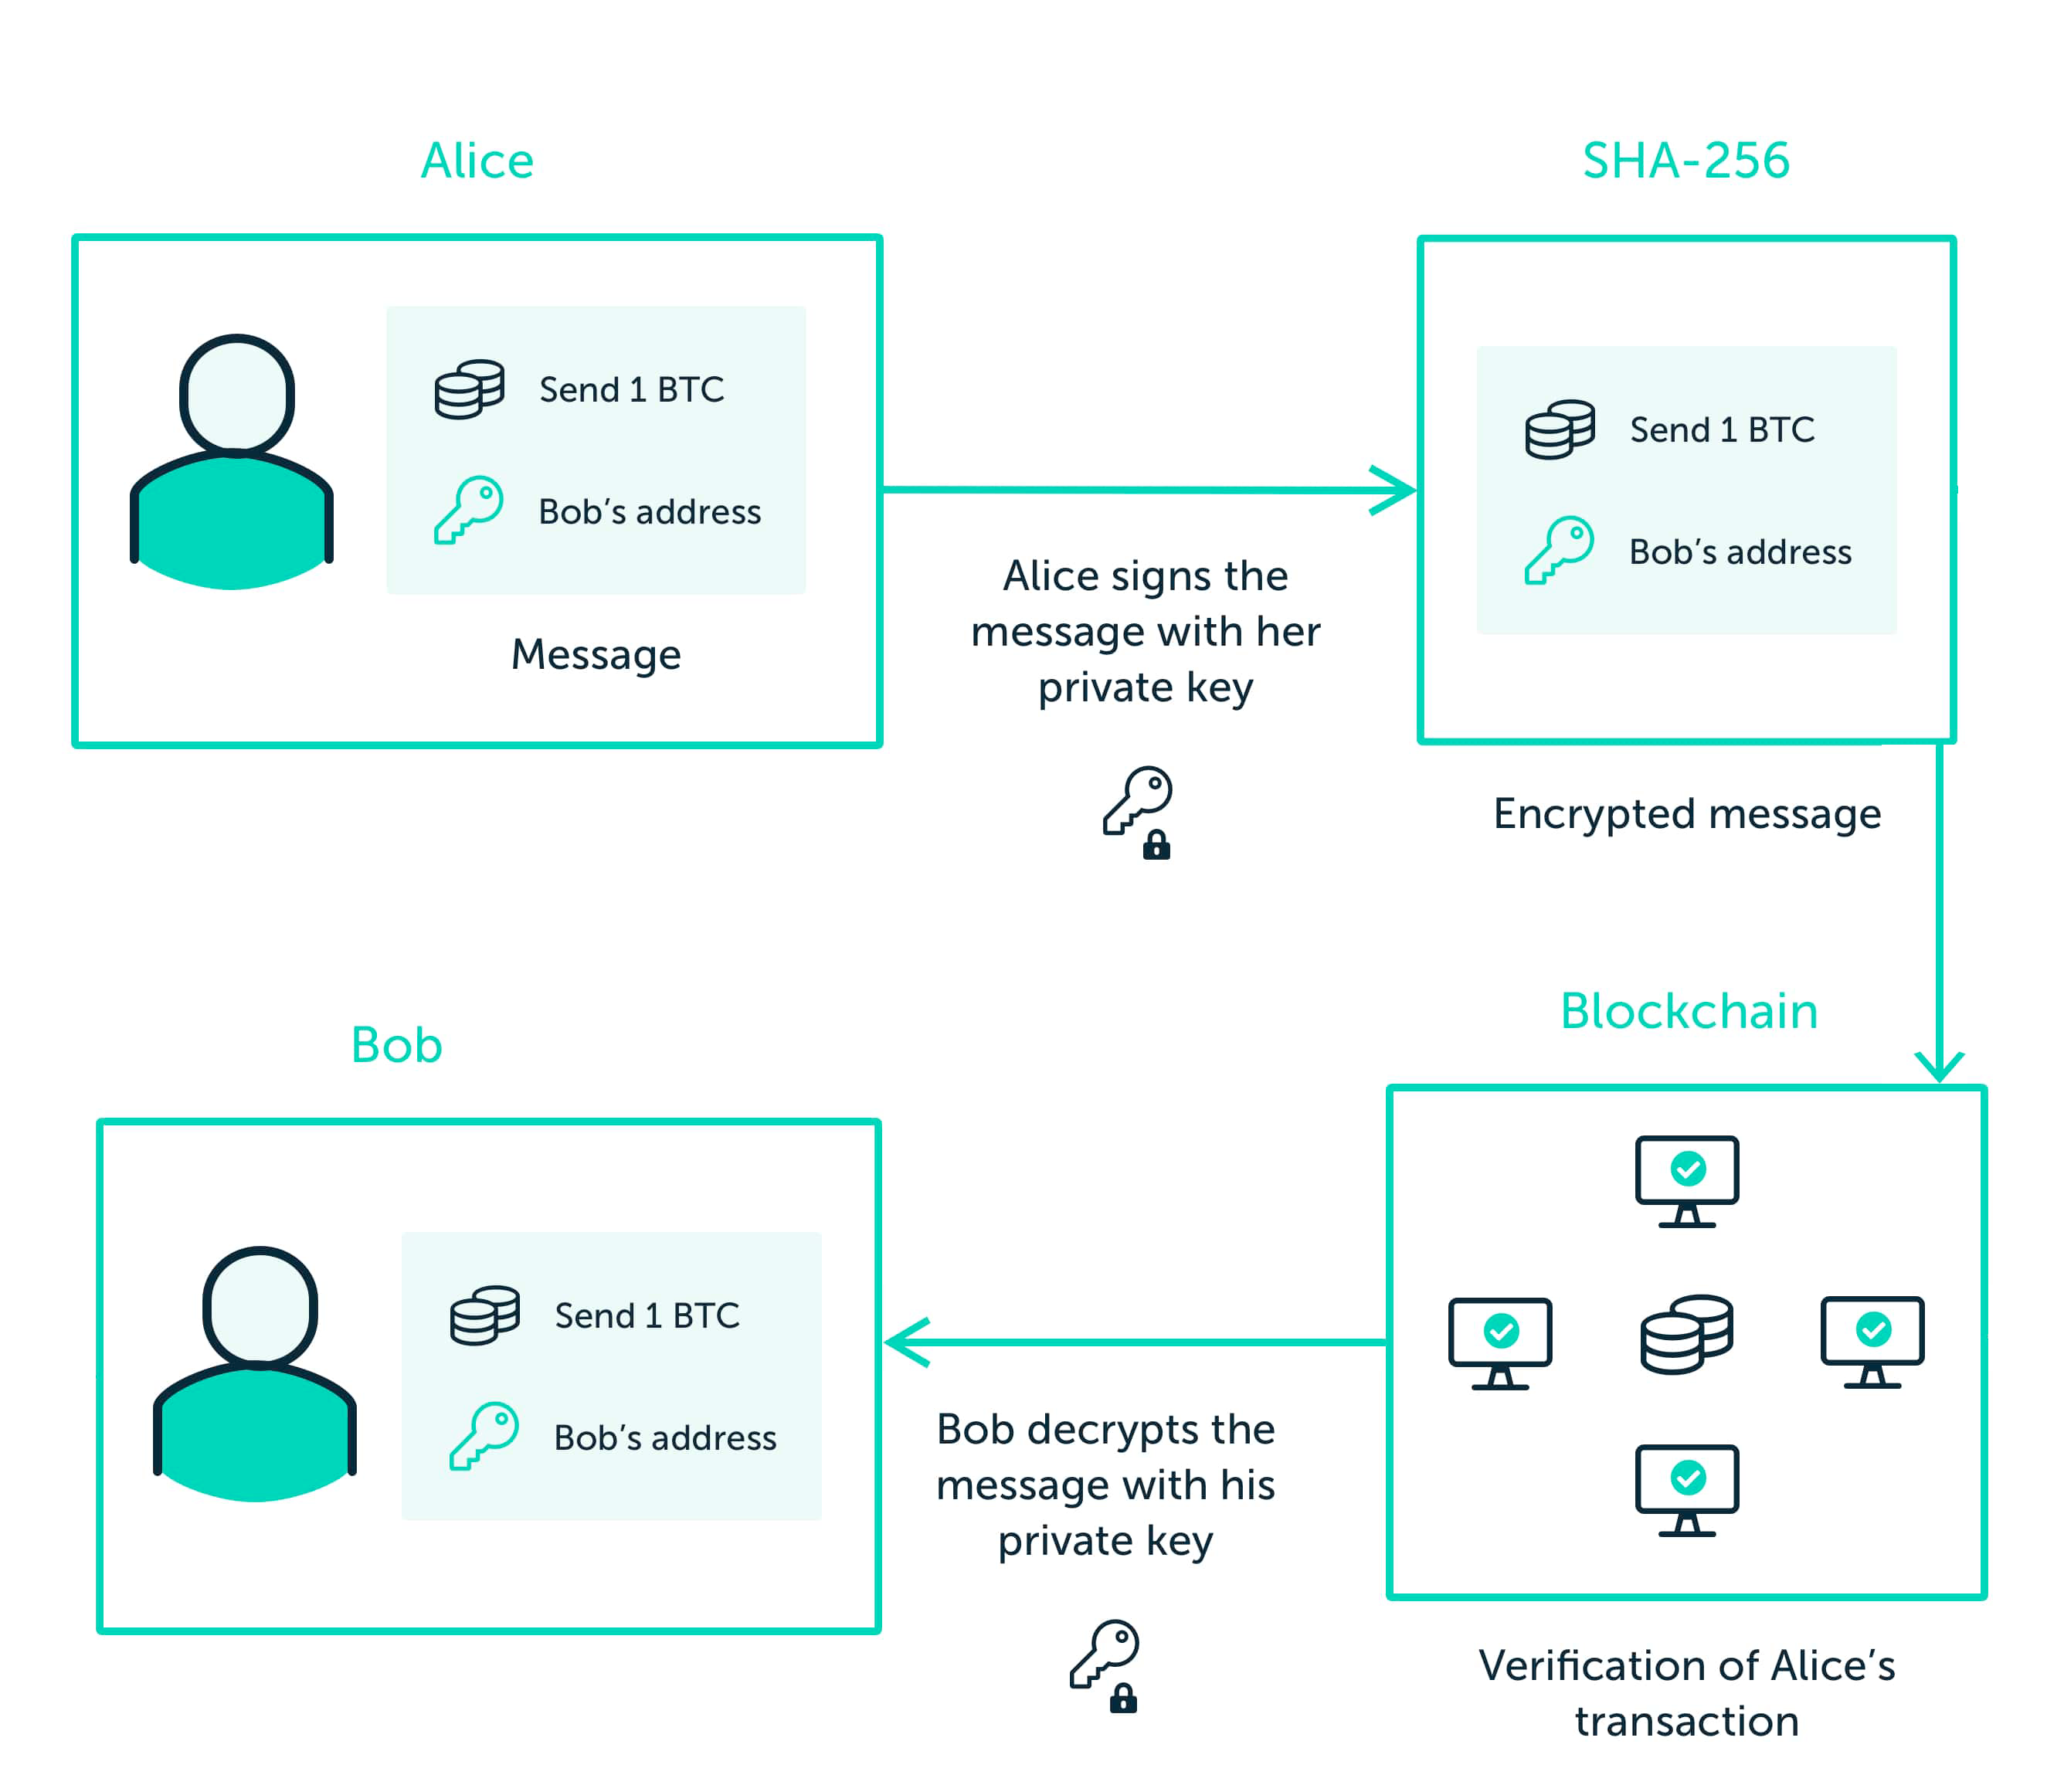
\includegraphics[scale=0.15]{images/PrivatePublicKeys}
\caption{Esempio di  \emph{transazione}}
\label{fig:privatePublicKeys}
\end{figure}

I \textit{wallet} sono dei sistemi sicuri che permettono di tenere riservate ed esclusivamente a conoscenza solo del creatore una o più chiavi private.
Inoltre, spesso forniscono informazioni utili come il bilancio, uno storico delle transazioni e molto altro.

La generazione di un wallet, con il suo indirizzo pubblico corrispondente, inizia con la creazione di una chiave privata a 64 caratteri (64 hexadecimal) casuali.
In seguito con un algoritmo basato sulle curve ellittiche (ECDSA) verrà generata la chiave pubblica. Essendo un algoritmo di cifratura asimmetrica, non è possibile, o computazionalmente molto complesso risalire alla chiave privata tramite la chiave pubblica. \cite{ledger-privatekey}

Infine, l'indirizzo del destinatario utilizzato per le transazioni è una forma rappresentativa della chiave pubblica, e prende il nome di \textit{address}.
In analogia al mondo reale si potrebbe dire che la chiave privata è il pin che permette l'accesso al proprio conto in banca, mentre la chiave pubblica l'indirizzo IBAN. \cite{blockchain-chiavi}

In generale, i wallet sono suddivisi in due principali categorie, \textit{Custodial} e \textit{Non custodial}.

I wallet di tipo custodial sono controllati da terze parti, in questo caso l'utente si affida alla sicurezza di questa terza parte per proteggere i propri fondi. Diversamente,  i wallet non custodial consentono agli utenti di mantenere il controllo delle proprie chiavi, senza doverle condividere con nessuno. Questo rende i non custodial wallet più sicuri rispetto ai wallet custodial, ma richiedono una maggiore competenza tecnica per gestirli correttamente.

In aggiunta, i wallet possono essere separati ulteriormente, tra la categoria di wallet fisici oppure basati su software.
I wallet basati su software hanno una maggior connessione ad internet e sono solitamente installati su computer utilizzati per vari scopi, quindi più vulnerabili agli attacchi, mentre i wallet fisici sono offline e separati, quindi più sicuri.
I \textit{software-based wallets} possono essere \textit{web-based}, mobile o desktop. Mentre i \textit{physical wallets} possono essere \textit{paper wallets} o \textit{hardware wallets} come una chiavetta usb o un dispositivo Bluetooth. \cite{custodial-wallet}

\subsection{Criptovalute}
\label{sec:criptovalute}

Le criptovalute sono una forma di denaro digitale che utilizza la crittografia per garantire la sicurezza delle transazioni e il controllo della creazione di nuove unità di valuta. 
Esse vengono utilizzate per effettuare transazioni all'interno di una blockchain, come ad esempio il trasferimento di denaro da un utente ad un altro, senza la necessità di un intermediario. \cite{binance-cryptocurrency}

Ogni blockchain ha la propria criptovaluta nativa, alcune delle più famose per capitalizzazione di mercato sono \textit{Bitcoin} e \textit{Ethereum} che sommate raggiungono una capitalizzazione di mercato di circa 1.000 miliardi di dollari. \cite{coinmarketcap}

\subsubsection{Stablecoin}
Le Stablecoin sono particolari criptovalute progettate appositamente per mantenere un valore stabile, questo è possibile attraverso attività sottostanti, come valute fiat, materie prime oppure algoritmica. Esse mirano a limitare l'alta volatilità del mercato delle criptovalute, rendendole più adatte ai pagamenti. Per questo motivo, la domanda di valute stabili è in forte crescita in tutto il mondo. \cite{swiss-stablecoin}
Infatti, le stablecoin hanno attirato l'interesse delle autorità di regolamentazione in tutto il mondo grazie al loro mix unico di fiat e criptovalute. Poiché sono progettate per mantenere un prezzo stabile, possono facilitare transazioni internazionali ad alta velocità a basso costo. \cite{binance-stablecoin}

\newpage

\subsection{Meccanismi di consenso}
\label{sec:consensoDistribuito}
Nel seguente capitolo verranno tre meccanismi di consenso distribuito, i quali sono alla base delle blockchain.

\subsubsection{PoW}
\label{sec:PoW}
Utilizzato da Bitcoin e in precedenza da Ethereum il \textit{Proof of work (PoW)} o \textit{Mining} è un meccanismo che si basa sul lavoro computazionale di computer. 
Al riempimento di un blocco, il primo nodo che riuscirà a creare un hash che soddisfa dei vincoli e una \textit{difficulty} potrà condividere il nuovo blocco con gli altri nodi. Essi verificheranno che il nuovo blocco sia corretto. successivamente questo verrà aggiunto alla catena (blockchain). \cite{binance-pow}

Perciò, il lavoro dei miner è di riuscire a creare un hash con i dati presenti nel blocco.
Essendo il contenuto presente non modificabile, allo scopo di ottenere un hash diverso, è presente un valore variabile chiamato \textit{nonce} che ad ogni tentativo di hashing viene modificato.

Una volta che il nuovo blocco è stato validato, il miner che ha trovato l'hash corretto viene solitamente remunerato con delle criptovalute native alla blockchain. \cite{binance-pow}

Essendo un lavoro computazionale dispendioso, dove i piccoli miner non riusciranno mai a calcolare l'hash necessario per primi, possono unire le forze in delle \textit{mining pool}, dove più individui condivido il potere computazionale ed in caso di vincita si divideranno in maniera proporzionale il valore ottenuto. \cite{bitpanda-miningPool}

Parte della sicurezza di nel meccanismo di consenso PoW risiede nella difficoltà del calcolo di un nuovo hash, perciò si può confermare che finché è presente una distribuzioni omogenea dei validatori la rete è sicura.
Nel momento in cui, una singola entità riesca ad ottenere più del 50\% della capacità di calcolo totale nella rete (anche noto come \textit{hasing rate}), quest'ultima avrebbe una probabilità di riuscire a calcolare per prima il nuovo hash e verifando in autonomia il nuovo blocco, inserendo transazioni non veritiere. Questo è noto come \textit{51\% attack}. \cite{coindesk-51attack}

\subsubsection{PoS}
\label{sec:PoS}

Il \textit{Proof of stake (PoS)} è un meccanismo di consenso dove i validatori dei nuovi blocchi sono selezionati in base alla quantità di criptovalute che hanno in \textit{staking}.
Il termine staking si riferisce al processo in cui gli utenti bloccano una quantità di criptovaluta per partecipare alla validazione dei blocchi sulla blockchain. In cambio del loro contributo, ricevono ricompense nella criptovaluta nativa al termine di ogni validazione. Questo processo aiuta a mantenere la sicurezza e la decentralizzazione della rete. \cite{vitalik-pos}

In contrasto al PoW, nel PoS quando un blocco deve essere validato, viene scelto un validatore in base ad una metodologia prefissata. Alcuni esempi sono: selezione random, random ma con probabilità proporzionale ai coin in stake, basato su anzianità, … \cite{ethereum-pos}
    
Il validatore scelto invierà la nuova versione della blockchain con il nuovo blocco validato e solo dopo la conferma degli altri nodi validatori la blockchain verrà aggiornata. \newline 
Nel meccanismo di PoW la tempistica di aggiunta di un nuovo blocco può essere variabile, vista la difficoltà di creare l'hash, mentre per il PoS il tempo di ogni nuovo blocco è prefissato. \cite{ethereum-pos}

Inoltre, in questo meccanismo di consenso è più redditizio compiere il proprio lavoro in modo onesto, dato che in caso di tentativo di truffa con la proposta di un blocco non valido viene inflitta una punizione. \cite{vitalik-pos}

Il validator può essere punito tramite uno \textit{slashing}, dove vengono detratti parte dei coin in stake oppure tramite un \textit{jailing}, nel quale il validatore viene messo in una blacklist e per un periodo di tempo non potrà effettuare il suo lavoro.
In aggiunta, quando un validatore vorrà finire la sua mansione è previsto un tempo prefissato di uscita, così che possa essere verificato che abbia svolto correttamente il suo compito. \cite{vitalik-pos}

\subsubsection{PoA}
I meccanismi di \textit{Proof of Authority} (PoA) sono una famiglia di algoritmi di consenso per permissioned blockchain (blockchain usate in ambiti privati alle quali si può accedere solo tramite invito). \cite{permissioned-blockchain}
L'importanza di questi meccanismi di consenso è data dal miglioramento delle performance rispetto agli algoritmi BFT; questo come risultato di uno scambio meno intenso di messaggi. \cite{PoA-paper} 

Gli algoritmi PoA si basano su un set di nodi detti \textit{authorities}.
Questi sono identificati da uno unique id e sono scelti arbitrariamente da un'entità fidata. A differenza degli algoritmi PoS, lo staking non avviene tramite coin ma attraverso la reputazione stessa del validatore.
Il consenso è determinato dall'unanimità di \textit{N/2 + 1} validatori, dove \textit{N} rappresenta la grandezza del loro set.
Dal momento che i nodi validatori sono a loro volta entità fidate, i meccanismi PoA offrono una resistenza eccellente a \textit{51\% attack}. 
Questo perché, a differenza dei meccanismi PoW dove un'entità malevola deve riuscire ad ottenere il 51\% della potenza computazionale della rete, in un meccanismo PoA un attaccante deve ottenere il controllo del 51\% dei nodi. \cite{51_attack_PoA} 

Questa famiglia di algoritmi non si basa sulla soluzione di puzzle, come accade per i meccanismi di consenso PoW, pertanto non richiede una attrezzatura altamente performante. Oltre a necessitare di meno potenza energetica e di calcolo, ha una maggiore velocità di validazione. \cite{51_attack_PoA}

La difficoltà nel selezionare nodi fidati rappresenta una forte limitazione per i meccanismi PoA, che a causa del ridotto insieme di validatori risultano essere efficienti solo all'interno di blockchain private. L'utilizzo di tali algoritmi per il consenso in blockchain decentralizzate è quindi sconsigliato.



\subsection{Ethereum}

Una delle principali blockchain è Ethereum. Come Bitcoin e altre criptovalute, offre la possibilità di trasferire valute digitali. 
Ad ogni modo, è capace di molto di più: è una tecnologia general purpose in grado di creare app e organizzazioni, detenere risorse e comunicare senza sottostare al controllo di un'autorità centrale. \cite{what-is-ethereum}

Ethereum è stata lanciata nel 2015 e differisce da Bitcoin per la possibilità di essere programmabile. 
È così possibile creare applicazioni decentralizzate chiamate Dapp mediante l'utilizzo di Smart Contract. Questi concetti saranno approfonditi più avanti nel documento. 

La criptovaluta nativa di Ethereum è chiamata ether (ETH) e possiede le proprietà tradizionali legate a un token, come l'essere decentralizzata e trasparente, necessarie per creare sistemi di finanza decentralizzata (DeFi).
Il modo più semplice per ottenere ETH è acquistarli tramite una delle molte piattaforme di scambio per criptovalute. \cite{what-is-ether}

Ogni azione sulla rete di Ethereum richiede una certa quantità di potenza di calcolo.
Questa commissione è pagata sotto forma di ether: ciò significa che serve almeno una piccola quantità di ETH per scrivere o modificare dei dati sulla rete, mentre l'operazione di lettura è priva di commissioni.

Ethereum non sottostà al controllo di alcuna entità e si basa unicamente sulla cooperazione della sua community.
Come altre blockchain, si basa su \textit{nodi}, sostituendo i tradizionali sistemi di server posseduti da grandi provider di Internet e servizi. Questa caratteristica di Ethereum rende l'infrastruttura estremamente resiliente, garantendo un altissima resistenza da attacchi. \cite{what-is-ethereum}

In aggiunta ai nodi già analizzati nel capitolo \hyperref[sec:blockchain]{\textit{Blockchain}}, Ethereum ha un tipo di nodo supplementare chiamato \textit{Archive node} che mantiene una copia completa della blockchain e di tutti gli stati passati. Invece, i \textit{Full node} mantengono una copia completa della blockchain e unicamente gli stati più recenti. \cite{ethereum-nodes}

Un'altra particolarità della blockchain Ethereum è la presenza di \textit{Ethereum Name Service (ENS)}. Questo permette di associare un nome leggibile (per esempio \textit{shopychange.eth}) ad un indirizzo Ethereum. Si tratta di un servizio molto simili al DNS, in quanto anch'esso lavora in una sistema gerarchico separato da punti. Il suo funzionamento è molto semplice, il registro ENS consiste in uno \hyperref[sec:smart-contract]{\textit{smart contract}} che mappa nomi di dominio a indirizzi Ethereum. \cite{ethereum-ens}

\subsubsection{Da PoW a PoS, merge e sharing}
Ethereum ha ufficialmente cambiato il proprio meccanismo di consenso distribuito il 15 settembre 2022 passando da PoW a PoS.
Il \textit{merge} ha permesso ad Ethereum di eliminare il processo di mining così da poter realizzare la loro vision: più scalabilità, sicurezza e sostenibilità. \cite{ethereum-vision}

\begin{figure}[ht]
    \centering
    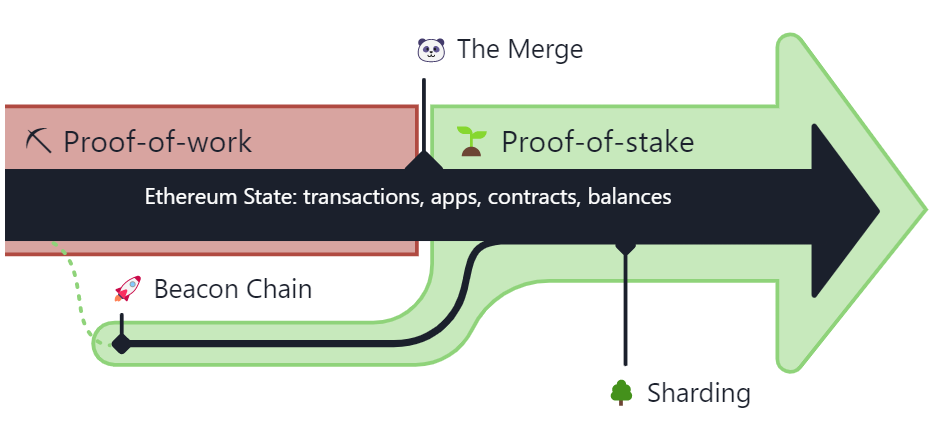
\includegraphics[scale=0.5]{images/ethereum-merge}
    \caption{Ethereum \emph{roadmap}}
    \label{fig:ethereum-roadmap}
\end{figure}

Il meccanismo PoS è stato introdotto già dal 1 dicembre 2020 nell'ambiente Ethereum.
Da questa data una blockchain chiamata \textit{Beacon Chain} ha lavorato in parallelo alla \textit{Mainnet PoW}, come è mostrato dalla Figura \ref{fig:ethereum-roadmap}, senza però validare transazioni.\cite{ethereum-pos} Dopo test intensivi, è avvenuto il merge dove la \textit{Beacon Chain} è subentrata come \textit{Blockchain} principale di Ethereum.
Il merge ha permesso ad Ethereum di diminuire di circa il 99.95\% l'energia consumata e di ottenere una migliore sicurezza. \cite{ethereum-merge}

Dal punto di vista degli utenti e holders l'interazione con l'ambiente Ethereum è rimasta invariata. 

Inoltre, essendo il tempo necessario per la validazione di un blocco non più dipendente da un lavoro computazione è ora fisso a 12 secondi. \cite{ethereum-merge} 

Il merge ha inoltre portato la possibilità di nuovi aggiornamenti e tecnologie al network.

Come la tecnica di \textit{Sharding} che è attualmente in fase di sviluppo e consentirà di aumentare la scalabilità di Ethereum permettendo di processare più transazioni in parallelo, ottendendo un risultato di più di 100'000 transazioni al secondo.
Lo Sharding permette di suddividere la rete ethereum in Shard, ovvero frammenti della blockchain principale in cui ogni shard gestirà un sottoinsieme di transazioni e di stato del sistema. Questo significa che la rete Ethereum risulterà più veloce e i sistemi sviluppati su di essa permetteranno un utilizzo più efficiente. \cite{ethereum-sharding}

\subsubsection{Ethereum Virtual Machine}

A differenza di altre blockchain, Ethereum offre la possibilità di definire ed eseguire degli \textit{smart contracts}, programmi informatici che risiedono e operano sulla blockchain.
Per questo funzionamento è necessario un componente specifico: la Ethereum Virtual Machine, o più semplicemente EVM.
Questa entità è una macchina a stati che definisce le regole per cambiare stato tra un blocco all'altro.
L'EVM non è altro che un computer virtuale, basato su un vasto insieme di computer distribuiti. \cite{ethereum-virtual-machine}

In Ethereum, uno stato è una grande struttura di dati chiamata \textit{Merkle Patricia Tree}, la quale mantiene tutti gli account collegati da hashes ed è riducibile a un singolo hash radice salvato sulla blockchain.
La macchina a stati di Ethereum processa le operazioni in modo sequenziale, e ad ogni transazione eseguita lo stato della EVM viene aggiornato.

La EVM si comporta come farebbe una funzione matematica: dato un input, produce un output deterministico.
Per eseguire operazioni, la EVM necessita di codice macchina.
Vista la difficoltà per un umano di programmare a un livello così sono stati sviluppati linguaggi di programmazione come \textit{Solidity}.
Questo è un linguaggio di programmazione \textit{object-oriented} disegnato appositamente per essere usato sull'Ethereum Virtual Machine.
La sintassi del linguaggio è stata influenzata da C++, Phyton e Javascript. \cite{solidity}
Il compito di Solidity e altri linguaggi di programmazione simili è quello di rendere la programmazione di \textit{smart contracts} più facile ed intuitiva tramite un linguaggio ad alto livello.


Una volta scritto il codice, questo viene compilato e tradotto in codice macchina.
Le operazioni da svolgere sono raggruppate in \textit{opcode}, un linguaggio intermedio tra linguaggio umano e linguaggio macchina.
Un opcode è un'operazione stack (XOR, AND, ADD, SUB ecc.) oppure un'operazione specifica per la blockchain (ADDRESS, BALANCE, BLOCKHASH ecc.).

\subsubsection{Gas e fees}
Dal momento che ogni operazione sulla EVM è molto dispendiosa in termini di tempo e risorse è stato inserito un meccanismo per prevenire che gli utenti usino la macchina a stati per operazioni di scarsa importanza.
Ad ogni opcode infatti corrisponde una determinata quantità di \textit{gas} per essere eseguito.
Il gas rappresenta l'ammontare di sforzo computazionale necessario per eseguire un'operazione specifica sul network Ethereum, e funziona come una tassa da pagare per eseguire del codice. \cite{gas-and-fees}

Il costo del gas è calcolato in \textit{gwei}, dove un gwei corrisponde a $10^{-9}$ ETH.
Anche il costo di una transazione è espresso in gwei ed è calcolato su una \textit{base fee} al quale si somma una \textit{priority fee}, la quale rappresenta una mancia per incentivare i \textit{miners} ad includere la transazione nel blocco.
Nel caso in cui si verifichino molte richieste nello stesso momento, i \textit{miners} saranno propensi ad includere nel nuovo blocco le transazioni con \textit{priority fee} maggiore: per questo motivo la quantità di gas necessaria per eseguire una transazione può variare.
È inoltre possibile specificare una \textit{max fee}, ovvero l'importo limite che si è disposti a pagare per eseguire una transazione.
La quantità di gas minima è determinata dal numero di operazioni di scrittura eseguite, creando la necessità di ridurre le informazioni da scrivere sulla \textit{Blockchain}.
Una soluzione per ridurre il numero di operazioni da scrivere e di conseguenza i costi delle transazioni è l'utilizzo di IPFS, trattati nel capitolo \hyperref[sec:ipfs]{\textit{IPFS}}.

Ogni istruzione di scrittura presente nella transazione consuma il gas totale fornito dall'utente.
Nel caso in cui un'istruzione necessiti di più gas rispetto a quello rimasto, l'esecuzione sarà interrotta e tutte le operazioni annullate.
Il gas consumato nell'esecuzione andrà perso, mentre quello rimanente sarà rimborsato all'utente.

\subsubsection{Mainnets e Testnets}
\label{sec:mainnet-testnet}

Nella tecnologia blockchain, una mainnet è lo stato finale, più stabile e completamente funzionale di un network blockchain.
Le mainnet offrono la possibilità di rilasciare DApps per l'utilizzo pubblico.
Tutte le transazioni reali sono eseguite sulla mainnet. \cite{testnet-vs-mainnet-shardeum}

Una testnet è un'istanza di una blockchain alimentata dalla versione medesima dello stesso software o più recente, con lo scopo di essere usata per fare testing e sperimentazione senza il rischio di dover esporre dei fondi reali o la chain principale (mainnet). \cite{testnet-wikipedia}

Data la natura immutabile di una blockchain, l'aggiunta di nuove features comporta dei rischi che possono portare a conseguenze anche catastrofiche, come la perdita dei fondi dei propri utenti.
Per questo motivo esperimenti rigorosi su una testnet sono spesso una buona pratica in termini di sicurezza.
Le criptovalute native alle testnet possono essere usate solo in tali blockchain e non hanno valore all'esterno della testnet.

Dal momento che il \textit{deploy} e la maggior parte delle operazioni su smart contracts hanno un costo in gas, e di conseguenza in valute reali, sviluppare una demo o un Proof of Concept su una mainnet comporterebbe costi non indifferenti.
In questo caso si può considerare l'uso di testnet che simuli il comportamento di una mainnet.
    
\paragraph{Sepolia}
Un esempio di testnet è Sepolia, una rete di test pubblica che funziona mediante la propria valuta (Sepolia ETH).
È stata creata nell'ottobre del 2021 dagli sviluppatori di Ethereum ed utilizza un meccanismo di consenso di tipo PoS.
Alcune particolarità di questa testnet sono i tempi di minig dei blocchi minori, che permettono di confermare le transazioni più velocemente, ed essere \textit{uncapped}.
Questa caratteristica implica che non esiste un limite al numero di coin che possono essere creati sulla testnet di Sepolia. \cite{sepolia}

Come per altre testnet, è possibile ottenere dei coin della blockchain tramite un Faucet, un'applicazione web che fornisce l'utente con una piccola quantità di criptovalute native.

\paragraph{Testnet locale}
Un altro metodo per testare le proprie applicazioni è quello di creare una testnet locale.
Questo metodo è particolarmente utile per testare le proprie applicazioni in un ambiente controllato, dove è possibile simulare diversi scenari e testare le proprie applicazioni in modo più approfondito.
Per creare una testnet locale è necessario installare un client Ethereum, come ad esempio Hardhat, e configurare il proprio ambiente di sviluppo. \cite{hardhat}

\subsubsection{Token}
Un token è un'unità digitale, rappresentata da un'entità unica su una blockchain, che può rappresentare una varietà di asset, come valute, proprietà, diritti di accesso, e così via.
Grazie alla loro programmabilità, i token possono essere utilizzati per creare applicazioni decentralizzate, effettuare transazioni finanziarie e gestire asset digitali in modo sicuro e trasparente. \cite{coinbase-token}

Inoltre, il termine \textit{token} è spesso usato come sinonimo di \textit{coin} ma non sono la stessa cosa.
Il termine \textit{coin} è un'alternativa a \textit{criptovaluta}, una moneta digitale basata su tecnologia blockchain, come spiegato in modo più approfondito nel capitolo \hyperref[sec:criptovalute]{\textit{criptovalute}}.
La differenza principale è il fatto che una coin è la moneta nativa della blockchain mentre i token sono altre monete che si appoggiano a smart contract.
Per esempio, ETH è la moneta nativa della blockchain ethereum mentre USDT (Tether) e BNB (Binance token) sono token.\cite{coinbase-token} 

\subsubsection{Smart Contract}
\label{sec:smart-contract}
Una delle principali caratteristiche che contraddistingue Ethereum è quella di poter definire smart contracts, programmi informatici che risiedono sulla blockchain.
Sono usati per creare \textit{Dapp}, applicazioni automatizzate che risiedono sulla chain e sono sempre pronte all'uso.

Uno smart contract è una raccolta di codice (definito dalle sue funzioni) e di dati (definiti dal suo stato) che risiede a un indirizzo specifico sulla blockchain Ethereum. 
Gli smart contracts sono un tipo di account Ethereum, per tanto possono essere l'oggetto di transazioni.
Nonostante questo, non sono controllati da un utente, ma sono distribuiti sulla blockchain ed eseguiti come programmato. \cite{smart-contracts}

Gli smart contracts sono scritti in un linguaggio di programmazione Turing completo, ovvero un linguaggio che può eseguire qualsiasi algoritmo. 
Il linguaggio più utilizzato per scrivere smart contracts è Solidity, un linguaggio di programmazione ad alto livello simile a Javascript. \cite{solidity}

La pubblicazione di uno smart contract necessita la compilazione del codice sorgente in bytecode, ovvero una rappresentazione del codice in linguaggio macchina. Durante la compilazione viene generato un \textit{Application Binary Interface (ABI)}, un file che contiene le informazioni necessarie per interagire con lo smart contract. \cite{smart-contracts}

Una volta che un contratto è pubblicato su Ethereum diventa visibile a tutti e non può più essere né modificato né rimosso.
Questa caratteristica serve a implementare il principio di \textit{Code is law}, una forma di regolazione dove la tecnologia è usata per imporre regole esistenti. \cite{code-is-law}

Alcuni casi d'uso degli smart contracts sono app di prestito, borse di credito decentralizzate, marketplace o crowdfunding.
Un particolare esempio di applicazione degli smart contracts è la creazione di NFT.
I Non-Fungile-Token sono degli assets digitali contraddistinti dalla loro unicità e dalla (quasi) impossibilità di essere contraffatti.
Dal momento che si basano sulla blockchain, cambiare il proprietario di un NFT o copiarne uno esistente sarebbe estremamente difficile e dispendioso. \cite{smart-contracts}

All'interno dei capitoli che seguono verranno approfonditi degli standard ERC (Ethereum Request for Comments), essi forniscono delle linee guida e specifiche tecniche per la definizione di un formato comune per la creazione di token su \textit{Blockchain} Ethereum. Gli standard ERC vengono proposti dalla \textit{community} di Ethereum che si occupa di discuterli e revisionarli. Lo scopo di questi standard è quello di garantire l'interoperabilità, la sicurezza e l'uniformità tra i diversi partecipanti della rete Ethereum. \cite{erc}

Sono state create diverse librerie con degli standard ERC già implementati, in modo da semplificare la fase di sviluppo e ridurre il rischio di errori. Un esempio di queste librerie è \textit{OpenZeppelin}\footnote{https://www.openzeppelin.com/}, la quale fornisce una vasta gamma di smart contracts già implementati, tra cui gli standard ERC20, ERC721 e ERC1155. \cite{ethereum-smart-contracts-library}

\paragraph{ERC20}
Lo standard ERC20 è fondamentale nell'ecosistema Ethereum. Esso permette la creazione di nuovi token fungibili e interscambiabili. La sua implementazione di base include la funzionalità di trasferimento da un account a un altro, senza la necessità di un intermediario. In aggiunta, lo standard ERC20 permette di ottenere il bilancio di un account e la supply totale del token, rendendo trasparente il funzionamento. \cite{erc20}


\paragraph{ERC721}
\label{sec:erc721}
Questo standard permette di identificare inequivocabilmente un bene ad una persona.
Infatti, lo standard ERC721 è ciò che rappresenta gli NFT, il quale viene identificato tramite un ID univoco.
Un NFT (Non-Fungible Token) è un tipo di token unico e irripetibile sulla blockchain, che rappresenta un asset digitale. 

In aggiunta, una collezione di NFT è un insieme di token che condividono lo stesso \textit{smart contract}, solitamente il creatore mantiene una coerenza tra i token della collezione, per esempio creando una collezione di immagini con lo stesso stile.

Grazie alla loro natura unica, gli NFT possono essere utilizzati per creare marketplace per asset digitali, per gestire diritti d'autore, per certificare l'autenticità di opere d'arte o di oggetti di valore, e molto altro ancora.

Questo standard ha un funzionamento di tipo modulare, dove ogni modulo è un contratto che implementa una funzionalità specifica. Più in dettaglio, lo standard ERC721 implementa le funzionalità di base per la creazione di un NFT e il trasferimento di proprietà dal proprietario o da un account autorizzato. Di seguito un elenco dei moduli aggiuntivi:

\begin{itemize}
    \item \textit{ERC721Metadata}: permette di aggiungere metadati al token, come il nome, la descrizione e l'immagine. Essi \textit{non} sono salvati nella blockchain in quanto risulterebbero troppo costosi, la soluzione più comunemente adottata è quella di salvare i metadati su \hyperref[sec:ipfs]{\textit{IPFS}} e salvare unicamente l'hash risultate sulla blockchain.
    \item \textit{ERC721Enumerable}: permette di migliorare la numerazione di NFT e la appartenenza ad un account, rendendo più facile la gestione di collezioni di NFT.
    \item \textit{ERC721Full}: Combinazione dei moduli ritenuti essere l'implementazione minima per un NFT, ovvero \textit{ERC721}, \textit{ERC721Metadata} e \textit{ERC721Enumerable}.
    \item \textit{ERC721Mintable}: Aggiunge la possibilità di creare nuovi token al di fuori del momento di creazione dello smart contract, aggiungendo inoltre un controllo su chi può creare nuovi token.
    \item \textit{ERC721Burnable}: Aggiunge la possibilità di distruggere un token, rimuovendolo dalla blockchain.
    \item \textit{ERC721Pausable}: Aggiunge la possibilità di mettere in pausa il contratto, impedendo il trasferimento di token.
\end{itemize}

Attualmente gli NFT sono spesso legati ad immagini, tuttavia essendo che i metadati sono solitamente salvati su \hyperref[sec:ipfs]{\textit{IPFS}}, è possibile creare NFT per qualsiasi tipo di asset digitale, come video, musica, documenti, oggetti 3D e molto altro. \cite{erc721}


\paragraph{ERC1155}
\label{sec:erc1155}

Lo standard ERC1155 è stato concepito per risolvere alcune problematiche presenti negli standard ERC20 e ERC721, come il costo di distribuzione (deploy) e la scalabilità. Una delle sue caratteristiche distintive è la possibilità di coniare sia token fungibili che non fungibili all'interno dello stesso contratto intelligente. Inoltre, l'ERC1155 ha introdotto un meccanismo innovativo che consente il trasferimento di più token attraverso una singola transazione, portando a una notevole riduzione delle spese di gas. Questa norma si dimostra estremamente vantaggiosa per lo sviluppo di dApp che richiedono una combinazione di token fungibili e non fungibili, ampliando notevolmente l'orizzonte delle possibilità nell'ambito delle applicazioni blockchain. \cite{erc1155}

\paragraph{ERC2981}
\label{sec:erc2981}
Questo standard consente di impostare un importo di \textit{royalty}, cioè una percentuale sulla vendita da pagare al creatore dell'NFT o ad un account scelto. Il pagamento deve essere messo in atto ogni volta che l'NFT viene venduto. L'ERC2981 è un estensione applicabili agli standard precedentemente analizzati, ovvero l'ERC721 e l'ERC1155. La motivazione che ha richiesto la creazione di questo standard è stata la la necessità di un meccanismo standardizzato per il pagamento delle \textit{royalty} all'interno dei marketplace. Tuttavia, il pagamento delle \textit{royalty} è un'operazione che richiede un'azione volontaria da parte del mercato digitale. 

Attualmente, la gestione delle \textit{royalty} non è unificata ed ogni marketplace ha il proprio sistema per gestire le \textit{royalty} creando diversi disagi di interoperabilità tra i vari marketplace. Lo standard ERC2981 fornisce un semplice meccanismo per risalire alla percentuale di \textit{royalty} da pagare, in modo da poter automatizzare il pagamento di esse. \cite{erc2981}

Attualmente, questo standard presenta la possibilità di inserire un solo destinatario per le \textit{royalty}, tuttavia potrebbe essere nell'interesse del creatore di una collezione di NFT di dividere le \textit{royalties} tra più persone. Per risolvere questo problema viene spesso utilizzato uno \textit{smart contract} che si occupa di dividere i pagamenti tra più destinatari, chiamato \textit{Payment Splitter}. \cite{payment-splitter}

\newpage

\subsection{IPFS}
\label{sec:ipfs}
Come precedentemente discusso nel capitolo \hyperref[sec:erc721]{\textit{ERC721}}, è spesso necessario conservare dati al di fuori del contesto della blockchain. Questa necessità deriva dal fatto che ogni singola informazione archiviata sulla blockchain comporta dei costi associati alla sua creazione. In questo contesto, l'archiviazione di dati tramite la rete IPFS (InterPlanetary File System) risulta essere una soluzione efficace per diminuire i costi di implementazione e contemporaneamente evitare un eccessiva espansione della rete blockchain.

L'IPFS rappresenta un insieme di protocolli utilizzati per l'organizzazione e il trasferimento efficiente dei dati. La sua struttura si basa su:
\begin{itemize}
    \item \textit{content addressing}: un metodo per individuare i dati utilizzando hash crittografici anziché basarsi sugli indirizzi IP.
    \item \textit{peer-to-peer networking}: un sistema di computer in cui ogni partecipante ha pari capacità ed è in grado di iniziare una sessione di comunicazione.
\end{itemize}

All'interno dell'infrastruttura IPFS, i dati sono suddivisi in blocchi, a cui avviene assegnato un identificatore univoco chiamato \textit{Content Identifier (CID)}, come già discusso precedentemente il CID è un hash crittografico che identifica univocamente un basandosi sul suo contenuto. In questo modo, ogni blocco può essere identificato in modo univoco e, se necessario, recuperato dalla rete IPFS. Inoltre, tramite l'utilizzo di CID, è possibile verificare l'integrità dei dati, infatti, se anche un singolo bit del blocco viene modificato, il CID cambia completamente. In aggiunta, è possibile ottenere un CID per una cartella, in questo caso il CID è calcolato in base ai CID dei blocchi che la compongono. Quest'ultima funzionalità risulta essere molto utile in collaborazione con lo standard ERC721Metadata, analizzato nel capitolo \hyperref[sec:erc721]{\textit{ERC721}}. \cite{ipfs}

Essendo IPFS un sistema peer-to-peer, i dati sono distribuiti tra i nodi della rete beneficiando di una maggiore disponibilità e ridondanza. Questo permette di avere un sistema più affidabile e resiliente rispetto ad un sistema centralizzato. Infatti, IPFS risulta essere un valido strumento utilizzato in parallelo alle reti blockchain, in quanto, come già precedentemente elencato, permette di ridurre i costi di archiviazione e allo stesso tempo consente di mantenere un alto livello di affidabilità. \cite{ipfs}